% !TeX root = ../thuthesis-example.tex

\chapter{绪论}

\section{研究背景与意义}
近年来,多媒体网络应用种类和业务量呈现爆发式增长的趋势,常见的应用场景包括流式视频点播、视频会议直播、云游戏视频、远程手术和360$^{\circ}$视频等。据统计,以云游戏为代表的业务量在2024年至2028年的复合年增长率将达到 33.59\% \cite{Global-Cloud-Gaming-Market-Size}。这类应用服务将成为网络流量的重要贡献者。应用种类的更新和业务量的增加使这类应用对网络传输的总体性能要求日益提升。作为重要的网络流量控制协议组件,网络传输速率控制策略(Rate Control Strategy) 在多媒体网络应用收发数据时承担发送速率控制、网络拥塞控制和避免、流式码率控制的重要角色。它们在网络传输瓶颈下对不同的网络指标,包括传输往返时延、丢包率、抖动、带宽利用率上作出取舍和权衡。速率控制的系统架构如图\ref{fig:teaser_system_archi}所示,控制策略即工作在左侧的发送端上,根据汇总的信息做出发送速率的决策。


\begin{figure} [ht]
\centering
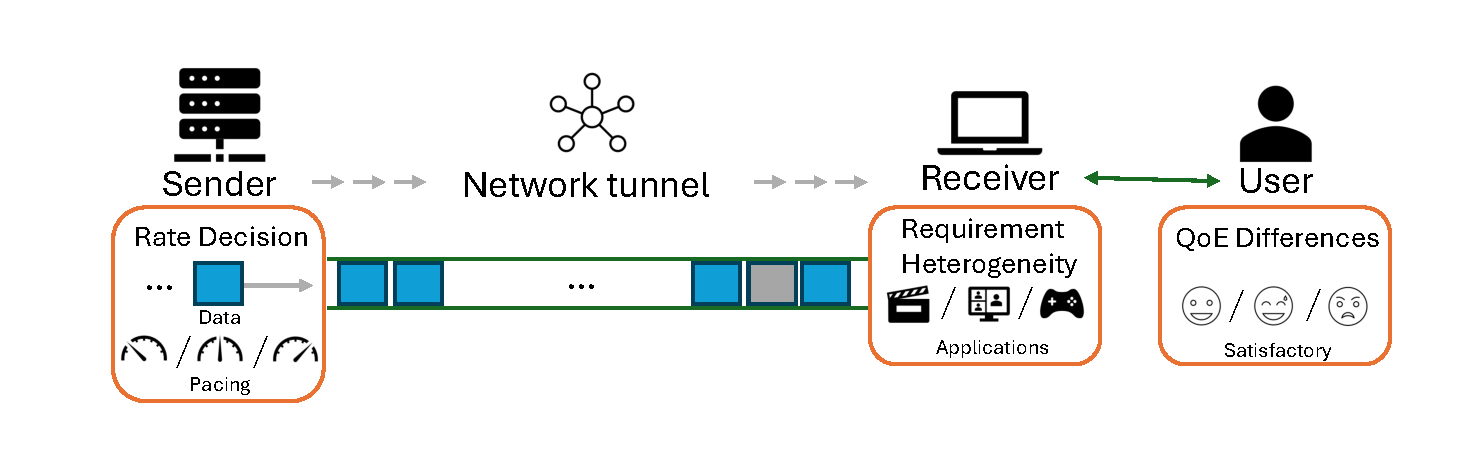
\includegraphics[width=\textwidth]{figures/chap01/system_archi.pdf} 
\caption{网络传输速率控制的系统架构}
\label{fig:teaser_system_archi}
\end{figure}


随着应用场景种类的增多,服务目标和用户偏好的分化造成了网络媒体应用对网络传输需求的异质性增加。例如流式视频点播的服务目标是在避免视频重新缓冲致使停顿的同时,尽力提升画面清晰度;视频会议直播的服务目标是保证低时延,与面对面交流反应时延的一致;云游戏视频的服务目标是保证用户交互反馈时延与本地游戏的一致性;远程手术需保证网络的稳定和可靠性;360$^{\circ}$视频的服务目标是视点内容的画面高清晰度。利用网络媒体应用对网络传输需求的异质性作出针对性的优化能够降低传输信息冗余,提升同等投入下的服务质量。若忽视服务目标的差异性而提供同质化的控制策略,也将折损用户体验质量(Quality of Experience,QoE)\cite{zhang2019e2e}。因此,网络媒体应用对网络传输需求的异质性已是策略设计中不可忽视的重要问题。

另一方面,传输速率控制策略经过了几十年间研究者的探索和积累,已经形成了庞大的可用策略库。这些策略由于具有差异的设计原理,呈现出对于不同的网络环境适配的差异性。例如,WestWood\cite{casetti2002tcp}被用于在无线网络下工作,POLYCORN\cite{ni2023polycorn}用于连接不稳定的网络下工作,Copa\cite{arun2018copa}用于超低时延环境下工作。传输速率控制策略的性能适配差异性为不同特性的网络环境提供潜在的选择。

然而,现存的传输速率控制策略面对网络传输需求的异质性和网络环境所需的性能适配差异性时,无法提供针对性优化。造成这种不足的原因是这些算法不具备感知应用场景并了解服务目标的能力,以及无法针对异质化的应用场景确定一个可量化的优化目标,为控制算法的针对性优化带来了困难。除此以外,现有的网络传输速率控制工作范式(Paradigm)通常采用固定的策略选择,无法利用上庞大的可用策略库。

% 一张图阐明 策略差异 以及 应用需求差异

在以上背景下,本文旨在设计一个可感知场景异质性的策略及一个新的传输速率控制范式,能够使策略感知具体网络媒体应用对网络传输需求,并根据感知的网络环境特性切换策略,提升传输信息的对用户体验的增益。

\section{研究挑战与内容}
现存的网络传输速率控制策略在面对传输异质化的应用场景时,缺乏对场景和用户偏好的定量感知能力和能利用感知结果的差异化控制策略;网络传输控制工作范式亦存在对所有网络状况和网络特性采用固定的策略选择的缺陷,造成了相同瓶颈网络条件下用户体验的次优。本文认为,用户体验的次优可以通过重新设计一个能够感知场景和用户偏好的策略以及利用上过去几十年累积的庞大的可用策略库来进行体验提升。具体的研究内容如图\ref{fig:final_goal}所示,其主要思想是利用两个环节的异质性和差异性,从两个角度切入优化速率控制模块,提升服务质量。

\begin{figure} [ht]
\centering
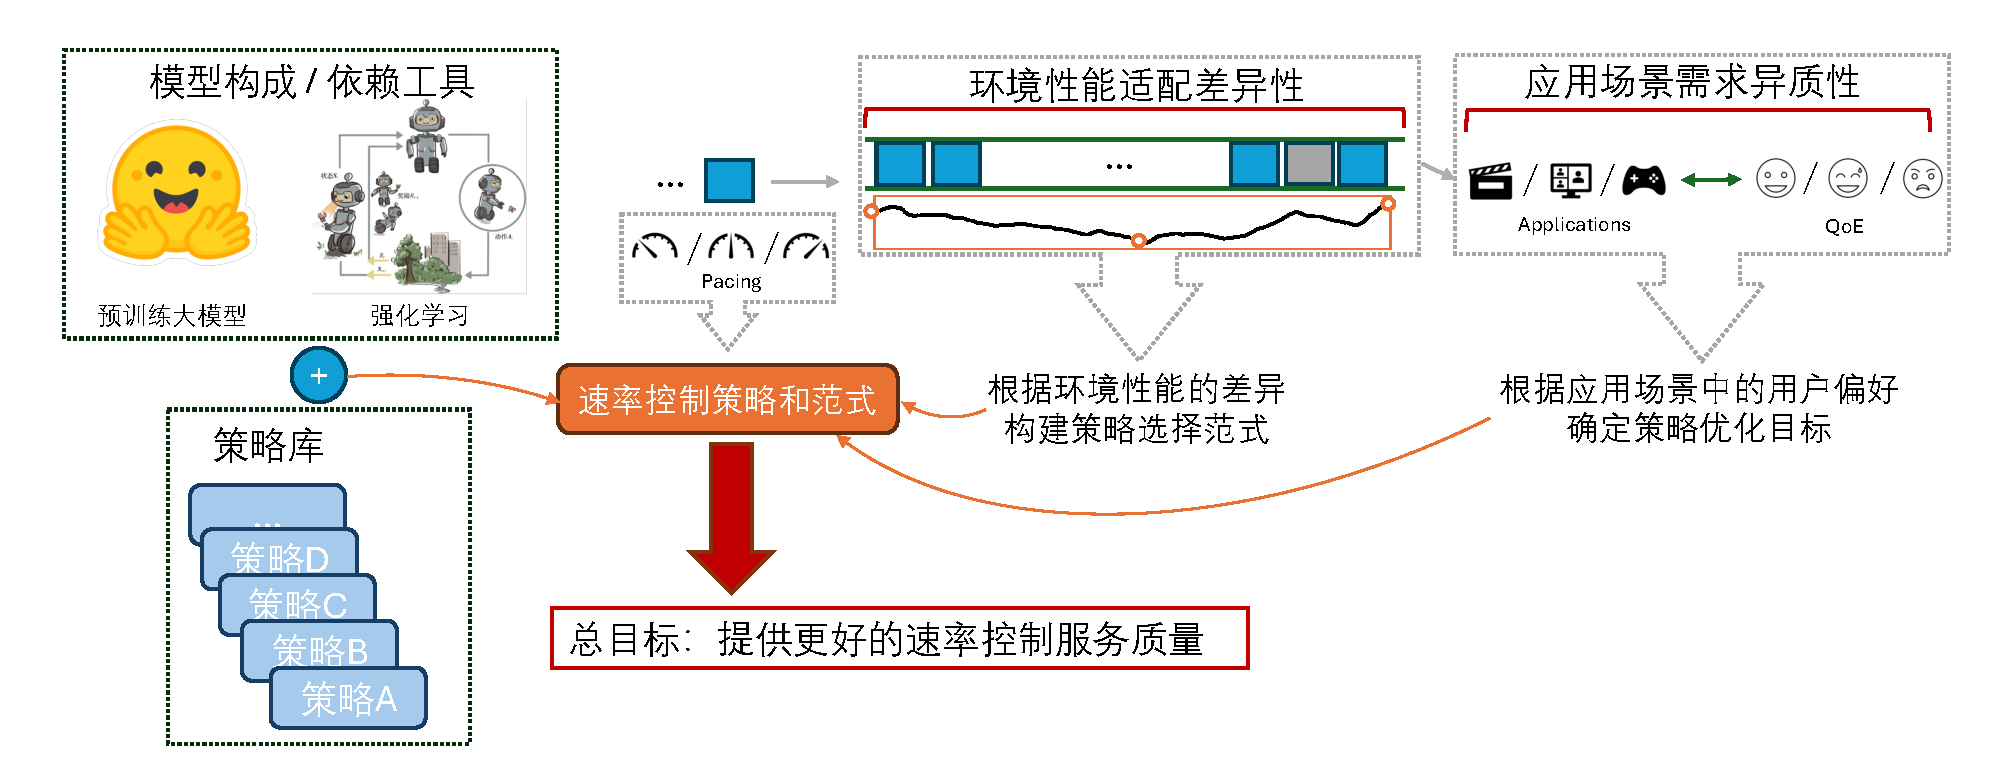
\includegraphics[width=\textwidth]{figures/chap01/final_goal.pdf} 
\caption{研究内容与框架}
\label{fig:final_goal}
\end{figure}


然而,实现服务的提升与速率控制质量改善的总目标需要解决以下挑战:
\begin{itemize}
    \item \textbf{如何根据应用场景中的用户偏好确定策略优化目标:} 网络传输需求的异质性使不同的应用场景有不同的优化目标。尽管根据用户需求能够直观地提供场景的定性分析(例如需要低时延或高吞吐量等),但是定性分析的结果难以作为某一策略的优化目标,需要可量化的方程式才可供算法进行最优解的迭代。然而,确定一个能直接反馈特定场景传输偏好的量化公式,需要对应场景下的用户反馈映射为网络指标的函数表达式。确定用户偏好至策略优化目标函数的映射方式是重要挑战。
    
    \item \textbf{如何设计可对场景感知的传输速率控制算法:} 传输速率控制算法需要具备对应用场景内容感知的能力,并将感知结果作用于算法的工作模式或参数调整上。对应用场景的感知需要依赖可靠的感知指标和能够进行特征提取的感知方法。传输速率控制算法在多影响因素(应用场景变化和网络波动)中,通过与外界环境感知和交互达到优化目标的最优解是一个复杂的决策任务。

    \item \textbf{如何利用累积策略库构建网络任务规划范式:} 现有的网络协议在建立连接后可动态切换策略的能力,因此要实现可切换策略的控制范式需要重定义工作流程,增加对宏观网络运行环境特性的感知,并支持策略库中策略切换。策略库的构建和更新需要范式具备提取策略工作特性和优点的能力。
    
\end{itemize}

本文着重讨论了应用场景下网络传输需求的异质性和策略环境适配的差异性的问题,旨在优化传输信息的对用户体验的增益。基于以上挑战,研究内容主要包括以下两个方面:

(1) 用户时延敏感度可感知的场景化传输速率控制算法

针对于网络传输需求的异质性,本文提出“时延敏感度”的概念,并旨在将时延敏感度通过数学方法映射为量化的函数,将此函数作为强化学习速率控制方法的优化目标,训练出不同场景下的最优解。通过开展针对真实用户场景下的评分测试获取用户满意与特定场景下网络指标之间关系的数据,解决上述的第一个挑战;随后设计基于强化学习的传输速率控制算法,使用流式画面内容编码器提供的信息作为场景感知信息,在高度波动的网络环境下结合场景特性和用户敏感性完成传输速率的控制,解决上述第二点挑战。本研究内容提供一种在带宽受限的情况下微调延迟和流式传输质量之间权衡的内容敏感方法。该研究内容的核心理念是在有限的带宽内,根据用户实验确定的延迟影响体验范围,在延迟和流式传输视觉质量之间取得平衡,从而提升用户体验质量(Quality of Experience,QoE)。由于云游戏设计多种场景,本工作在云游戏的多个差异化场景下展开测量和评估。

(2) 具备策略库的网络任务规划范式设计

针对于策略环境适配的差异性,本文旨在提出一个新范式,能够将过去网络控制策略选择范式中固定和对所有连接统一的固定策略,不会灵活更换的设计方案作出更新化迭代。为了将过去数几十年的算法构成可供备选的策略库,需要学习到策略所适配的网络特性和算法特点,形成可以根据网络环境特性作出最佳选择的范式。为了实现对历史策略的学习,构建策略切换的流程和作出选择决策,本研究内容包括对网络传输通信的控制协议流程进行重新设计,使其支持控制策略切换;网络策略的选择则需要感知网络特性,选择合适的策略,该研究内容解决了上述第三点挑战。近年来大模型可以作出决策的能力涌现,包括对环境理解的能力、推理和决策能力。因此本研究内容将使用预训练大模型进行网络控制策略选择范式设计。

\section{研究主要贡献}
本文的主要贡献点如下:

(1) 设计了一个可对场景中用户偏好感知的云游戏下实时通信传输速率控制算法。该算法首先通过对用户开展主观打分实验获得平均意见分数(Mean Opinion Score,MOS),确定了不同的应用场景下的三种敏感度类型,并使用了最小二乘估计(Least Square Estimation,LSE) 的数学方法估计拟合高、中、低敏感度的延迟感知敏感度曲线。算法将敏感度曲线作为奖励函数,使用Actor-Critic 架构强化学习速率控制算法为不同的时延敏感度场景量身定制,有助于实现延迟和视觉质量之间的更好平衡,从而使 QoE 提高高达 16.7\%。为了减少对于用户敏感度主观评分的依赖,此算法还使用来自视频流的信息,即时间感知信息 (Temporal perceptual Information,TI) 和空间感知信息 (Spatial perceptual Information,SI) 对游戏的敏感度进行分类,准确率达到 89\%。

(2) 重构了具备累积策略的网络任务策略规划范式构。该算法通过对现有的传输速率控制范式进行流程重定义,改变了过往在网络传输控制中固定一成不变的策略,增加了一个连接建立前的网络特性探测机制,使用预训练大模型(Pretrained Language Model,PLM)的感知与规划能力,为差异化的网络环境和连接流提供选用不同的策略的潜在可能性;通过在模拟环境下采集多个已有策略的工作模式和工作流程确定了方法适配的网络环境,并对预训练大模型(LLaMA)增加时序感知的嵌入(Embedding)模块,使用低秩矩阵分解(Low-Rank Adaptation,LoRA)的方法对大模型的输出进行微调和对齐,提升大模型选择策略和参数的有效性和成功率。该方法成功建立一个稳定和不易出错,且有效地利用上策略差异性提升网络传输速率控制质量的范式,超越了传统范式中单一算法在波动的网络环境中的运行性能。


\section{论文组织结构}
本文一共包含五个章节,图\ref{fig:arrange}展示了每个章节的内容。第二章概述了现有的网络传输速率控制策略在解决传输需求的异质性和策略环境适配的差异性的相关工作,包括对现有速率控制策略的总结与分类、对于传输需求的异质性的研究工作总结和利用策略环境适配的差异性的范式总结,以及方法所涉及强化学习框架的介绍。
第三章主要介绍场景时延敏感度可感知的传输速率控制,包括对用户偏好的量化感知方法和强化学习速率控制方法的设计。
第四章主要介绍具备策略库的⽹络任务规划范式设计,包括对范式工作流程的设计方法和对应的网络控制流程训练时大模型的微调对齐方法。
第五章对本文的研究内容进行总结,并对未来的研究方向作出展望。

\begin{figure} [ht]
\centering
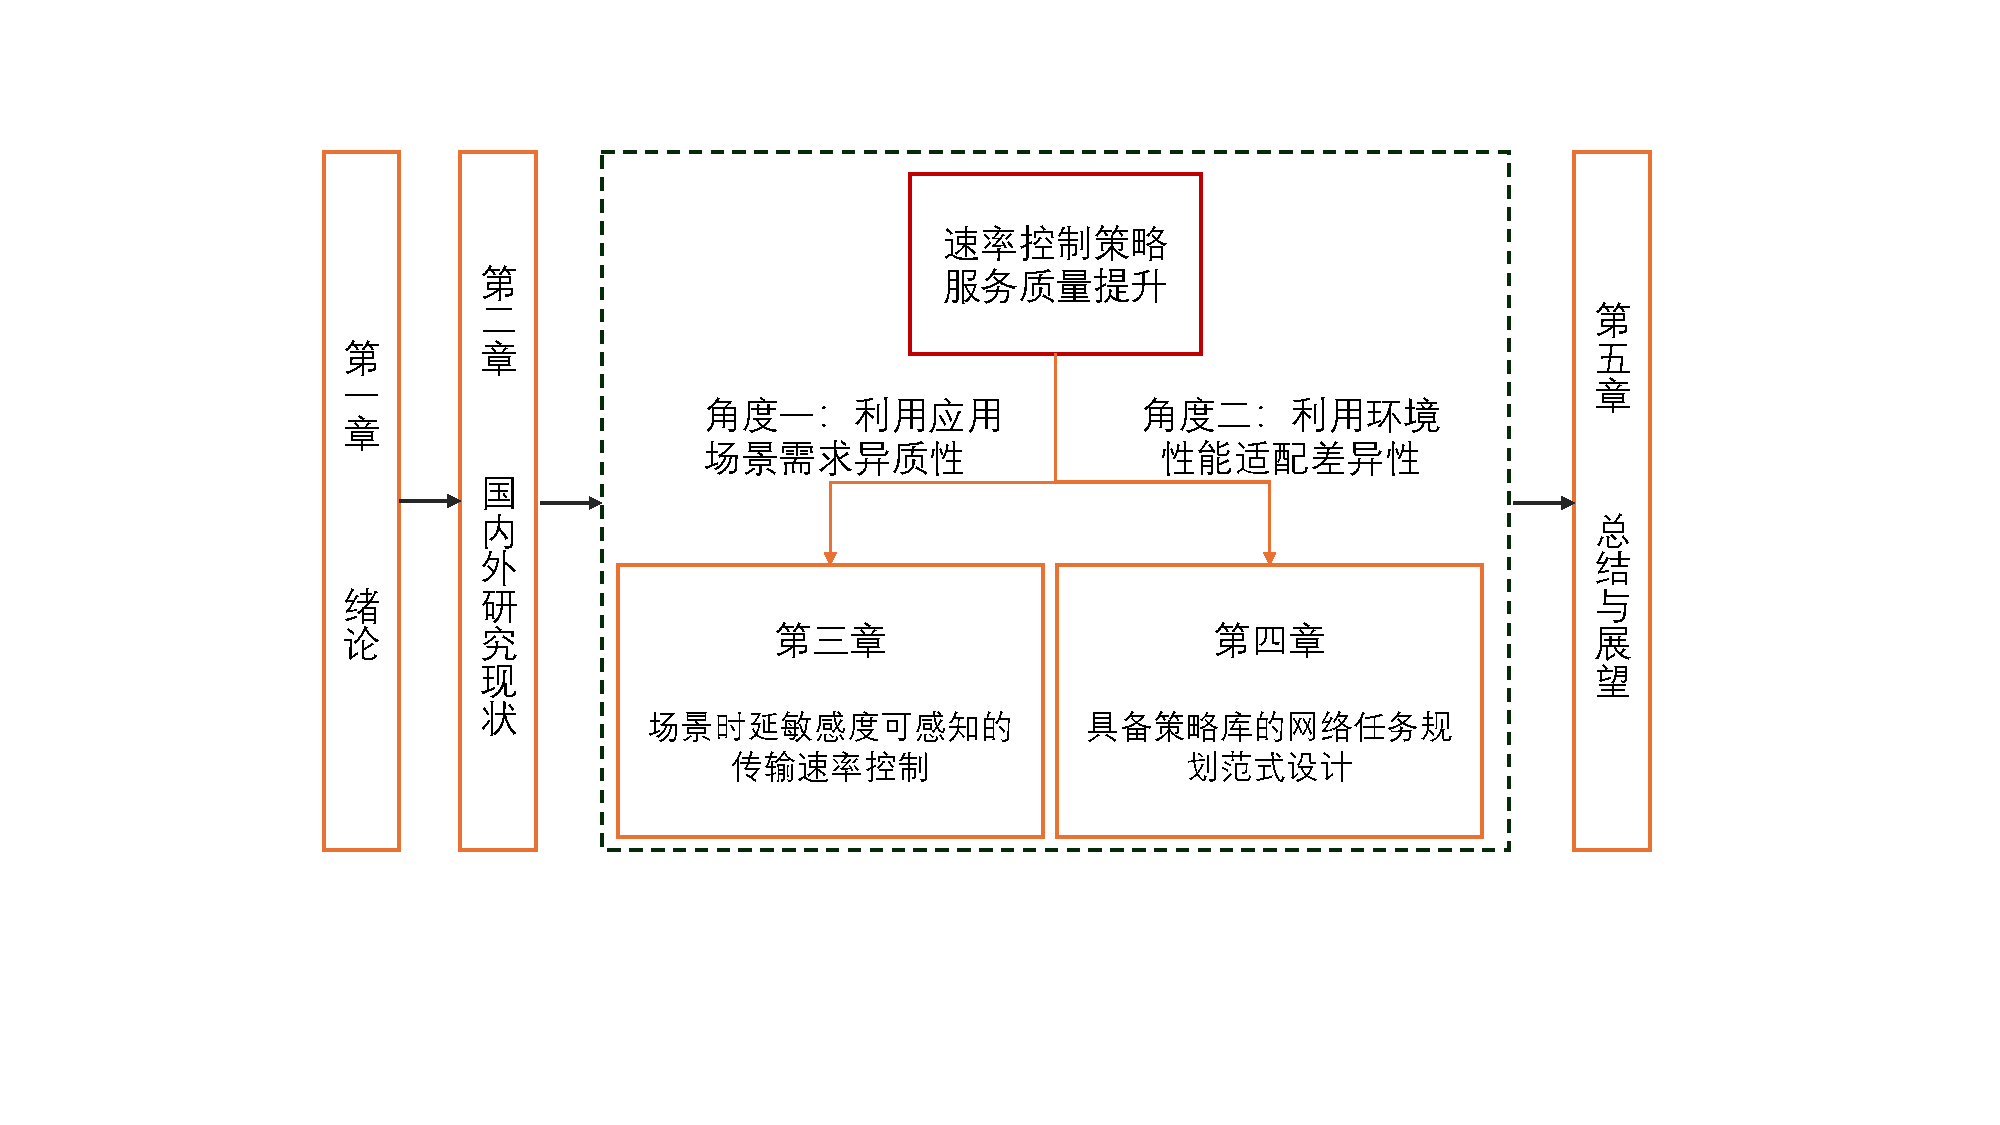
\includegraphics[width=0.8\textwidth]{figures/chap01/arrange.pdf} 
\caption{本文各章内容安排与结构}
\label{fig:arrange}
\end{figure}
